% vim: set tw=78 tabstop=4 shiftwidth=4 aw ai:

\chapter{Protocol Measurements in Peer-to-Peer Systems}
\label{chapter:proto-measure}

Based on BitTorrent's success story (it has managed to become the number one
protocol of the internet in a matter of years), the scientific community has
delved heavily in analysing, understanding and improving its performance.
Research focus has ranged from measurements~\cite{measurement-study} to
protocol improvements~\cite{bt-impr}, from social
networking~\cite{tribler-social} to moderation
techniques~\cite{measurements-analysis}, from content distribution
enhancements~\cite{bitos} to network infrastructure impact~\cite{bt-impact}.

We undertook a novel approach involving client-side information collection
regarding client and protocol implementation. We have instrumented a
libtorrent-rasterbar
client\footnote{http://www.rasterbar.com/products/libtorrent/} and a
Tribler\footnote{http://www.tribler.org/trac/} client to provide verbose
information regarding BitTorrent protocol implementation. These results are
collected and subsequently processed and analysed through a rendering
interface.

\todo{BitTorrent specification}
\todo{focus on real world measurements}
\todo{collect and analyze}

Swarm measured data are usually collected from trackers. While this offers a
global view of the swarm it has little information about client-centric
properties such as protocol implementation, neighbour set, number of connected
peers, etc. A more thorough approach has been presented by Iosup et
al.~\cite{corr-overlay}, using network probes to interrogate various clients.

Our approach, while not as scalable as the above mentioned one, aims to collect
client-centric data, store and analyse it in order to provide information on
the impact of network topology, protocol implementation and peer
characteristics. Our infrastructure provides micro-analysis, rather than
macro-analysis of a given swarm. We focus on detailed peer-centric properties,
rather than less-detailed global, tracker-centric information. The data
provided by controlled instrumented peers in a given swarm is retrieved,
parsed and stored for subsequent analysis.

We differentiate between two kinds of BitTorrent messages \textit{status
messages}, which clients provide periodically to report the current session’s
download state, and \textit{verbose messages} that contain protocol messages
exchanged between peers (chokes, unchokes, peer connections, pieces transfer
etc.).

\section{Related Work}
\label{sec:proto-measure:related}

\todo{related work}

\section{Message Types}
\label{sec:proto-measure:message-types}

\todo{message types}
\todo{status, verbose}
\todo{internal information}
\todo{approaches on collecting information}
\todo{hook points}
\todo{data collection, archiving}

\section{A Generic Logging Library}
\label{sec:proto-measure:log-library}

\todo{hook points}
\todo{architecture}
\todo{output types}
\todo{clients tested}

\section{Log Collecting and Parsing}
\label{sec:proto-measure:log-collect-parse}

\todo{enable, update clients}
\todo{monitoring or post processing}
\todo{experiments}
\todo{data parsing architecture}
\todo{post parsing and real time parsing}
\todo{storage}

\section{Monitoring}
\label{sec:monitoring}

Client monitoring is enabled trough the use of
MonALISA\footnote{http://monalisa.cern.ch/monalisa.htm}. MonALISA-specific
scripts are used to provide required information to the central repository.
The is typically invoked every 5 seconds. The service station collects
required information and sends them to the monitoring repository.

\begin{figure}[h]
  \begin{center}
    \includegraphics[width=0.7\textwidth]{src/img/proto-measure/monalisa-monitoring}
  \end{center}
  \caption{Monitoring with MonALISA}
  \label{fig:proto-measure:monitoring}
\end{figure}

Figure~\ref{fig:proto-measure:monitoring} is an architectural view of the
monitoring infrastructure. The core component of the monitoring framework is
the MonALISA service. The service is able to discover other monitoring
services and to be discovered by interested clients. Each service registers
itself with a set of Lookup Services (LUSs) as part of a dedicated monitoring
group and it publishes a set of dynamic attributes that describe it. This way
any interested application can request specific services based on a set of
matching attributes.

The service consists of an ensemble of multi-threaded subsystems,
which carry out several functions in an independent fashion, being able to
operate autonomously. Some of the most important functions it
performs are:

\begin{itemize}
  \item monitoring of a large number of entities (hosts running BitTorrent
  test scenarios) using simultaneously several modules which interact actively
  with the entities or passively listen for information, or interface with
  other existing monitoring tools;
  \item filtering and aggregation of the monitoring data, providing additional
  information based on several data series;
  \item storage for short period of time of the monitoring information, in
  memory or in a local database; this way, clients can get also history for
  the monitoring information they are interested in, not only the real-time
  monitored values; web services for direct access to the monitored data, from
  the monitoring service; local clients can get the information directly,
  without following the whole chain;
  \item triggers, alerts and actions based on the monitored P2P information,
  being able to react immediately when abnormal behaviour is detected;
  controlling using dedicated modules allow performing more complicated
  actions, that cannot be taken only to the local flow of information. This
  way, the service can act based on monitoring information from several
  services at the command of a controlling client, or direct or indirect users
  request.
\end{itemize}

The repository collecting monitoring information from the service is basically
a database. Information can be rendered through a web interface, or by using
the MonALISA interactive client interface. The monitoring data repository
offers long history for a few, preconfigured parameters related to BitTorrent
testing environment. The time series for these parameters are stored in a
database for long-term viewing purposes.

Due to the large amount of data (from all the services in community), the
typical usage is for storing aggregated and summary values. For those, it
offers a set of predefined charts in a web application format that allow
selecting among the set of time series and the time interval to plot. The data
repository client has been extended to support automated actions and alerts
based on some configurable triggers.

The two main functions of the data repository are adding new values and
querying the storage for data matching a given predicate. Particular
implementations are available for different purposes: plain text file logging
of data or database backends, values averaged in time or keeping original data
as it was produced, database structures optimized for keeping arbitrary
parameters or structures optimized for a well-known limited set of parameters.
All database-backed storage structures have the option to re-sample the values
on the fly, to provide a uniform time distribution of values.

New storage implementations that fit particular needs can be easily added. The
default database backend for all services is PostgreSQL. Both the Service and
the repository come with a precompiled PostgreSQL package that is used by
default, but the configuration parameters allow pointing to a different
backend. In addition to any permanent storage for the monitoring values a
volatile memory buffer is kept internally, serving as cache for recent data.
The size of this memory buffer is dynamically adjusted function of how much
memory was allocated to the Java Virtual Machine and how much of it is free.
This volatile storage is enough for running a light monitoring service, being
able to serve history requests in the limit of how much data the service was
able to keep in memory.

While the communication mechanism is shared with the interactive client and
the storage layer is the same as the one in the basic MonALISA Service, the
repository web interface is the particularity of this component. Built around
a Tomcat servlet engine and the JFreeChart charting library, the repository
offers a few powerful servlets that cover most of the known use cases: matrix
views of the values, bar, pie and histogram charts, geographical maps, scatter
plots etc. These views are easily configurable either by editing text files or
by using the web interface itself to create new views.

The repository can also act as a global aggregator. It has the same support as
the Service for running filters on the collected data, producing derived
values that can be stored along or instead of the original values. Custom
filters can be implemented to intercept received data (or particular cuts in
it) and act on the values. A particular kind of filters is the automatic
actions framework. Triggered by the monitored data values (comparison with
predefined thresholds, absence of data, arbitrary correlations or custom
pieces of code) automatic action be taken.

\section{Client Logging}
\label{sec:results-logging}

In order to examine BitTorrent transfer at a protocol implementation level, we
propose a system for storing and analysing logging data output by BitTorrent
clients. It currently offers support for
hrktorrent/libtorren and Tribler.

Data is provided by BitTorrent clients in log files that are parsed, stored,
interpreted and rendered. We have divided the information generated by clients
into \textbf{status log files} and \textbf{verbose log files}, each composed
of one of two types of messages.

\textit{Status messages} are periodic messages reporting session state.
Messages are usually output by clients at every second with updated
information regarding number of connected peers, current download speed,
upload speed, estimated time of arrival, download percentage, etc. Status
messages are to be used for real time analysis of peer behaviour as they are
lightweight and periodically output (usually every second).

\textit{Verbose messages} or \textit{log messages} provide a thorough
inspection of a client's implementation. The output is usually of large
quantity (hundreds of MB per client for a one-day session). Verbose
information is stored in client side log files and is subsequently parsed and
stored.

Our study of logging data takes into consideration two open-source BitTorrent
applications: Tribler and hrktorrent\footnote{http://50hz.ws/hrktorrent/}
(based on libtorrent-rasterbar. While the latter needed minimal changes in
order to provide the necessary verbose and status data, Tribler had to be
modified significantly.

The process of configuring Tribler for logging output is completely automated
using shell scripts and may be reversed. The source code alterations are
focused on providing both status and verbose messages as client output
information.

\textit{Status message} information provided by Tribler includes transfer
completion percentage, download and upload rates. In the modified version, it
also outputs current date and time, transfer size, estimated time of arrival
(ETA), number of peers, and the name and path of the transferred file.

In order to enable \textit{verbose message} output, we took advantage of the
fact that Tribler uses flags that can trigger printing to standard output for
various implementation details, among which are the actions related to
receiving and sending BitTorrent messages. The files we identified to be
responsible for protocol data are changed using scripts in order to print the
necessary information and to associate it to a timestamp and date. Since most
of the protocol exchange data was passed through several levels in Tribler's
class hierarchy, attention had to be paid to avoid duplicate output and to
reduce file size. In contrast to libtorrent-rasterbar, which, at each transfer,
creates a separate session log file for each peer, Tribler stores verbose
messages in a single file. This file is passed to the verbose parser, which
extracts relevant parts of the messages and writes them into the database.

Unlike Tribler, hrktorrent's instrumentation did not imply modifying its
source code but defining \texttt{TORRENT\_LOGGING} and
\texttt{TORRENT\_VERBOSE\_LOGGING} macros before building (recompiling)
libtorrent-rasterbar. Minor updates had to be delivered to the compile options
of hrktorrent in order to enable logging output.

The BitTorrent clients and log parsers are configured to distinguish between
the following protocol
messages\footnote{http://www.bittorrent.org/beps/bep\_0003.html}:
\begin{itemize}
  \item \textbf{choke} and \textbf{unchoke} -- notification that no data will
be sent until unchoking happens.
  \item \textbf{interested} and \textbf{not interested} -- notifies of a peer's
'interested'/'uninterested' state\footnote{Connections contain two bits of
state on either end: choked or not, and interested or not.}. Data transfer
takes place whenever one side is interested and the other side is not choking.
  \item \textbf{have} -- sent to inform all peers of a piece's successful
download (its hash matches the one from the .torrent metafile)\footnote{The
peer protocol refers to pieces of the file by index as described in the
metainfo file (.torrent file), starting at zero. Connections contain two bits
of state on either end - choked or not, and interested or not.}.
  \item \textbf{bitfield} -- sent after an initial handshaking sequence between
peers. The payload is a bitfield representing the pieces that have been
successfully downloaded.
  \item \textbf{request} -- sent to obtain blocks of data, the payload
contains a piece index and the block's length and offset within the piece.
  \item \textbf{piece} -- contains a block of data, its position within a piece
and the piece's index. By default these messages are correlated with request
messages, but there are cases when an unexpected piece arrives if choke and
unchoke messages are sent in quick succession and/or transfer is going very
slowly.
  \item \textbf{cancel} - cancels a request for a piece; it has the same
payload as the \textit{request} message. These messages are commonly used when
the download is almost complete; \textit{request} messages are sent to many
peers to make sure the final pieces arrive quickly; when a piece is
downloaded its other requests are cancelled.
\end{itemize}

Although our system processes and stores all protocol message types,
the most important messages for our swarm analysis are those related to
changing a peer's state (choke/unchoke) and requesting/receiving data.
Correlations between these messages are the heart of provisioning information
about the peers' behaviour and BitTorrent clients' performance.

\section{Data Processing Engine}
\label{sec:proto-measure:data-processing}

\todo{database schema, rendering}
\todo{monitoring and MonALISA goes here}

As client instrumentation provides in-depth information on client
implementation, it generates extensive input for data analysis. Coupled
with carefully crafted experiments and message filtering, this will allow
the detection of weak spots and of improvement possibilities in current
implementations. Thus it will provide feedback to client and protocol
implementations and swarm ``tuning'' suggestions, which in turn will enable
high performance swarms and rapid content delivery in peer-to-peer systems.

Currently, the infrastructure consists of the following modules:

\begin{itemize}
  \item \textbf{Parsers} -- receive log files provided by BitTorrent
clients during file transfers. Due to differences between log file formats,
there are separate pairs of parsers for each client. Each pair analyses status
and verbose messages.
  \item \textbf{Database Access} -- a thin layer between the database system and
other modules. Provides support for storing messages, updating and reading
them.
  \item \textbf{SQLite Database} -- contains a database schema with tables
designed for storing protocol messages content and peer information.
  \item \textbf{Rendering Engine} -- consists of a GUI application that
processes the information stored in the database and renders it using plots
and other graphical tools.
\end{itemize}

\begin{figure}[h]
  \begin{center}
    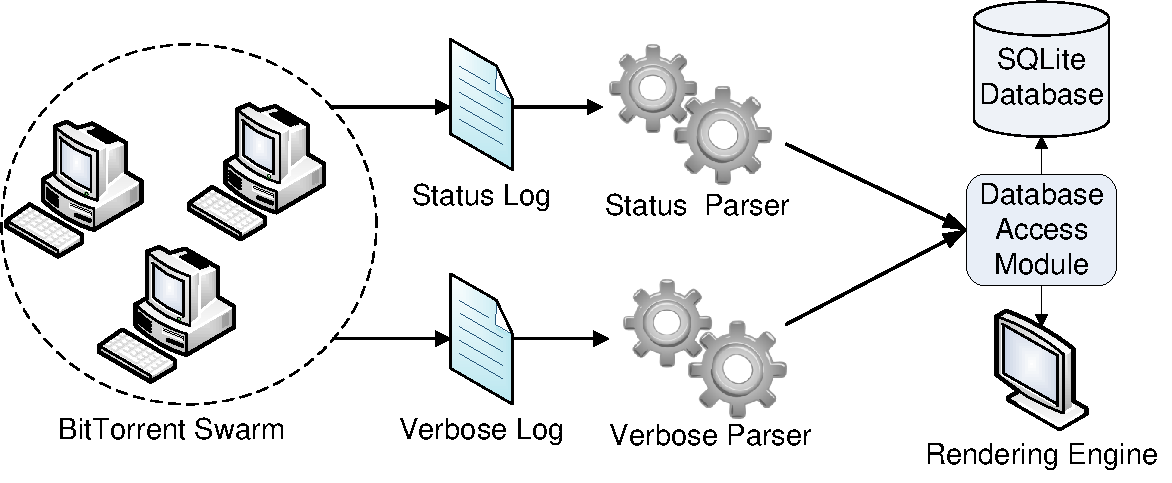
\includegraphics[width=0.7\textwidth]{src/img/proto-measure/logarch-not-use}
  \end{center}
  \caption{Logging System Overview}
  \label{fig:proto-measure:logarch}
\end{figure}

As shown in Figure~\ref{fig:proto-measure:logarch}, using parsers specific to
each type of logging file, messages are sent as input to the \textit{Database
Access} module that stores them into an SQLite database. In order to analyse
peer behaviour the Rendering Engine reads stored logging data using the
Database Access module and outputs it to a graphical user interface.

Once all logging and verbose data from a given experiment is collected, the
next step is the analysis phase. The testing infrastructure provides a GUI
(\textit{Graphical User Interface}) statistics engine for inspecting peer
behaviour. 

The GUI is implemented in Python using two libraries: \textit{matplotlib}
-- for generating graphs and \textit{TraitsUi} -- for handling widgets. It
offers several important plotting options for describing peer behaviour and
peer interaction during the experiment:

\begin{itemize}
  \item \textit{download/upload speed} -- displays the evolution of
download/upload speed for the peer;
  \item \textit{acceleration} -- shows how fast the download/upload speed of
the peer increases/decreases;
  \item \textit{statistics} -- displays the types and amount of verbose
messages the peer exchanged with other peers.
\end{itemize}

The last two options are important as they provide valuable information about
the performance of the BitTorrent client and how this performance is
influenced by protocol messages exchanged by the client.

The \textit{acceleration} option measures how fast a BitTorrent client is able
to download data. High acceleration forms a basic requirement in live
streaming, as it means starting playback of a torrent file with little delay.

The \textit{statistics} option displays the flow of protocol messages. We are
interested in the choke/unchoke messages.

The GUI also offers two modes of operation: \textit{``Single Client Mode''},
in which the user can follow the behaviour of a single peer during a given
experiment, and \textit{``Client Comparison Mode''}, allowing for comparisons
between two peers.

\section{Evaluating Peer-to-Peer Performance}
\label{sec:eval-swarm}

The virtualized infrastructure and automated framework provides the necessary
platform for experimental evaluation of Peer-to-Peer implementations and
formal models. Our interest resides in evaluating BitTorrent clients, which
mostly translates to sheer download speed; the higher the download speed, the
better the performance. Obviously, we have to take into account both peer
download speed and swarm download speed. A peer with high download speed that
more or less ``free rides'' on top of the other peers is not desired in a
given swarm.

In order to properly consider a formal evaluation mechanism for performance
evaluation of a Peer-to-Peer ecosystem, several questions must be answered:

\begin{itemize}
  \item What do we measure?
  \item What do we consider for evaluation?
  \item What do we vary? What is influencing the measurement?
  \item How do the above correlate?
  \item What do we consider to be ``better''?
\end{itemize}

The answer to the first question is given by data acquired from status and
verbose log files: protocol messages, number of connections, download and
upload speed, resource usage. This may be acquired through measurements,
monitoring and log files. As mentioned above, we will consider download speed
as an evaluation unit for performance. We consider the other measurable unit
to correlate to the download speed.

The units we may vary include:

\begin{itemize}
  \item hardware resources -- base or virtualized system resources such as
  RAM, CPU, I/O and networking;
  \item peer/system characteristics -- download speed limitation, upload speed
  limitation, connection limitation, existence of a firewall;
  \item Peer-to-Peer implementation -- software application and protocol
  design;
  \item swarm and network characteristics -- number of peers, network
  topology, peer connectivity, network bandwidth, etc.
\end{itemize}

The varying units influence the measured units. Though we will focus mostly on
download speed, the other units also provide influence. If a given peer
receives a boost in its upload speed that means it will also boost download
speed of sever other peers. If a given varying unit would directly influence
upload speed, that will also provide influence over download speed, though it
may not happen directly. It may be easier to detect influence of varying units
over secondary units, such as protocol messages.

As such, we consider a correspondence between varying units and measured
units:

\begin{align}
\label{eq:proto-measure:eval}
Eval(hw, sys, impl, swarm, net) = (protomsg, speed, conn, ruse)
\end{align}

Our goal is to maximize download speed translates in defining and/or adjusting
the most suitable values for the varying units. A proper implementation,
deployed in a proper environment will ensure increased performance.

This leaves answering the last question: \textit{What do we consider
``better''?}. High download speed roughly translated to low download time. In
order to achieve good/better performance, we required minimizing download
time. Download time is, however, a static unit: we only measure it at the end
of the given scenario. As it is influenced by download speed evolution that
is, in its turn, influenced by other factors, we aim to correlate download
time with the evolution of download speed.

If we were to continuously monitor download speed, a pure mathematical formula
for a given peer would be:

\begin{align}
  FS = \int_0^{DT} DS(t)\,dt
\end{align}

where:

\begin{itemize}
  \item FS -- file size
  \item DT -- download time
  \item DS -- download speed (evolution)
\end{itemize}

As we only periodically monitor a peer, the formula translates to:

\begin{align}
  FS = \sum_{t=0}^{DT} DS_{t}
\end{align}

This provides necessary correlation between download speed evolution and
download time, with the file size being well known.

In order to correlate download speed with other units, we have to consider
download speed as the interaction with other peers. A peer may only download
if other peers upload. We formalize this as a download matrix that may
be built for each interval of monitoring:

\begin{align}
  PDS_{t} =
  \begin{pmatrix}
    ds_{1,1} = 0 & ds_{1,2} & \cdots & ds_{1,NP} \\
    ds_{2,1} & ds_{2,2} = 0 & \cdots & ds_{2,NP} \\
    \vdots & \vdots & \ddots & \vdots \\
    ds_{NP,1} & ds_{NP,2} & \cdots & ds_{NP,NP} = 0 \\
  \end{pmatrix}
\end{align}

where:

\begin{itemize}
  \item $ds_{i,j}$ -- download speed of peer \texttt{j} from peer \texttt{i};
  \item \texttt{PDS} -- peer download speed matrix at time \texttt{t};
  \item \texttt{NP} -- number of peers in swarm;
\end{itemize}

Peer to peer download speed is easily measurable and as it fairly easy to
correlate it to varying units. Using an array of such matrices, a matrix
element for each time slice, one will possess detailed measured information
regarding peer download speed and, by summing up either rows, columns or the
whole matrix, provide the ability to observe peer upload speed, peer download
speed and swarm download speed.

The most important step, left as further work is to establish a formal
definition or approximation for Equation~\ref{eq:proto-measure:eval}. This
will allow the establishment of the most important units to be considered and
updated to ensure peer and swarm performance.
